%%%%%%%%%%%%%%%%%%%%%%%%%%%%%%%%%%%%

\section{Hypothesis testing}

%%%%%%%%%%%%%%%%%%%%%%%%%%%%%%%%%%%%

\subsection{Hypothesis testing framework}

%%%%%%%%%%%%%%%%%%%%%%%%%%%%%%%%%%%%

\begin{frame}
%\frametitle{Remember when...}

Gender discrimination experiment:

{\small
\begin{tabular}{ll  cc c} 
  		&				& \multicolumn{2}{c}{\textit{Promotion}} \\
\cline{3-4}
							&			& Promoted	& Not Promoted 	& Total	\\
\cline{2-5}
\multirow{2}{*}{\textit{Gender	}}	&Male 		& 21	 	& 3		& 24 	\\
							&Female		& 14	 	& 10 	 	& 24 \\
\cline{2-5}
							&Total		& 35		& 13		& 48 \\
\end{tabular}
}

\pause

\[ \hat{p}_{males} = 21 / 24 \approx 0.88 \]
\[ \hat{p}_{females} = 14 / 24 \approx 0.58 \]

\pause

Possible explanations:\pause
\begin{itemize}
\item Promotion and gender are \hl{independent}; there is no gender discrimination; observed difference in proportions is simply due to chance. $\rightarrow$ \orange{null} - {\small (nothing is going on)}
\item Promotion and gender are \hl{dependent}; there is gender discrimination, observed difference in proportions is not due to chance. $\rightarrow$ \orange{alternative} - {\small (something is going on)}

\end{itemize}

\end{frame}

%%%%%%%%%%%%%%%%%%%%%%%%%%%%%%%%%%%%

\begin{frame}
\frametitle{Result}

\begin{center}
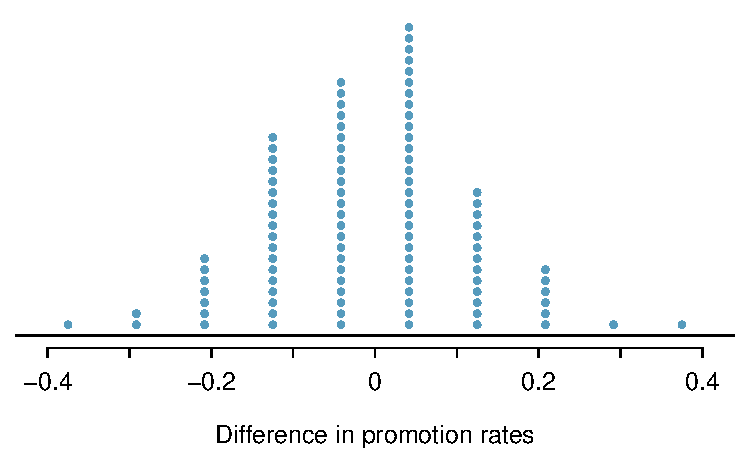
\includegraphics[width=0.75\textwidth]{4-3_hyp_test/figures/discRandDotPlot/discRandDotPlot}
\end{center}

\pause

Since it was quite unlikely to obtain results like the actual data or something more extreme in the simulations (male promotions being at least 30 percentage points higher than female promotions), we decided to reject the null hypothesis in favor of the alternative.

\end{frame}

%%%%%%%%%%%%%%%%%%%%%%%%%%%%%%%%%%%%

\begin{frame}
\frametitle{Recap: hypothesis testing framework}

\begin{itemize}
\item We start with a \hl{null hypothesis ($H_0$)} that represents the status quo. (Difference [of means or proportions] due to chance.)
\pause
\item We also have an \hl{alternative hypothesis ($H_A$)} that represents our research question, i.e. what we're testing for. (Difference due to association between variables.)
\pause
\item We conduct a hypothesis test under the assumption that the null hypothesis is true, either via simulation or traditional methods based on the central limit theorem (coming up next...).
\pause
%\item If the test results suggest that the data do not provide convincing evidence for the alternative hypothesis, we stick with the null hypothesis. If they do, then we reject the null hypothesis in favor of the alternative.
\item If the difference is unusual under the null, we reject the null. (Unusual is measured with $z$ score and tail area.) Otherwise, we retain the null.
\end{itemize}
\pause
We'll formally introduce the hypothesis testing framework using an example on testing a claim about a population mean.

\end{frame}

%%%%%%%%%%%%%%%%%%%%%%%%%%%%%%%%%%%%

\subsection{Testing hypotheses using confidence intervals} 

%%%%%%%%%%%%%%%%%%%%%%%%%%%%%%%%%%%%

\begin{frame}
\frametitle{Testing hypotheses using confidence intervals}
\vspace{-10pt}
{\small Earlier we calculated a 95\% confidence interval for the average number of exclusive relationships college students have been in to be (2.7, 3.7). Based on this confidence interval, do these data support the hypothesis that college students on average have been in more than 3 exclusive relationships.}

\pause

\begin{itemize}

\item The associated hypotheses are:
\begin{itemize}
\item[$H_0$:] $\mu = 3$: College students have been in 3 exclusive relationships, on average
\item[$H_A$:] $\mu > 3$: College students have been in more than 3 exclusive relationships, on average
\end{itemize}

\pause

\item Since the null value is included in the interval, we do not reject the null hypothesis in favor of the alternative.

\pause

\item This is a quick-and-dirty approach for hypothesis testing. However it doesn't tell us the likelihood of certain outcomes under the null hypothesis, i.e. the p-value, based on which we can make a decision on the hypotheses.

\end{itemize}

\end{frame}



\begin{frame}
\frametitle{example study}
On the Longfellow bridge, the speed limit is 25 miles per hour. A cycling advocate hopes to find evidence that cars speed on the bridge (but will look elsewhere if none exists... [this is a problem in research...]). The advocate decides to measure a random sample of car speeds and to apply a one-tailed test.\pause

What are the relevant hypotheses? \pause

\soln{null hypothesis, ~~$H_0$:~~ $\mu = 25$ } \pause 

\soln{alternative hypothesis, ~~$H_a$:~~ $\mu > 25$ }
\end{frame}

\begin{frame}
\frametitle{example study (fake data)}
The advocate takes a sample of 80 cars, which yield a sample mean of 28 miles per hour and a standard deviation of 15 miles per hour. Does the advocate have significant evidence of speeding? \pause

We wonder... maybe the true population mean is 25 mph and this sample mean of 28 mph is just due to natural fluctuation. \pause

So, we want to know how common/uncommon this difference is from random fluctuation alone. \pause

Luckily, sampling distributions are normal! So if we estimate that $\sigma \approx 15$ mph, we have everything we need to answer that question.
\end{frame}


\begin{frame}
\frametitle{Build the sampling distribution of the null hypothesis}
The null hypothesis suggests that the population parameters are $\mu = 25$ and $\sigma \approx 15$. \pause

What are the parameters of the null's {\bf sampling distribution}?
\soln{$$\mu = 25$$} \pause
\soln{$$SE = \frac{15}{\sqrt{80}} = 1.68$$}

\end{frame}


%%%%%%%%%%%%%%%%%%%%%%%%%%%%%%%%%%%%

%%\begin{frame}
%%\frametitle{Number of college applications}

%%\dq{{\small A similar survey asked how many colleges students applied to, and 206 students responded to this question. This sample yielded an average of 9.7 college applications with a standard deviation of 7. College Board website states that counselors recommend students apply to roughly 8 colleges.  Do these data provide convincing evidence that the average number of colleges all Duke students apply to is \emph{higher} than recommended?}}

%%\vfill

%%\ct{\webURL{http://www.collegeboard.com/student/apply/the-application/151680.html}}

%%\end{frame}

%%%%%%%%%%%%%%%%%%%%%%%%%%%%%%%%%%%%

%%\begin{frame}
%%\frametitle{Setting the hypotheses}

%%\begin{itemize}

%%\item The \hl{parameter of interest} is the average number of schools applied to by \underline{all} Duke students.

%%\pause

%%\item There may be two explanations why our sample mean is higher than the recommended 8 schools.
%%\begin{itemize}
%%\item The true population mean is different.
%%\item The true population mean is 8, and the difference between the true population mean and the sample mean is simply due to natural sampling variability.
%%\end{itemize}

%%\pause

%%\item We start with the assumption the average number of colleges Duke students apply to is 8 (as recommended)
%%\[ \mathhl{H_0:}~\mu = 8 \]

%%\pause

%%\item We test the claim that the average number of colleges Duke students apply to is greater than 8
%%\[ \mathhl{H_A:}~\mu > 8 \]

%%\end{itemize}

%%\end{frame}

%%%%%%%%%%%%%%%%%%%%%%%%%%%%%%%%%%%%%%%

%%\subsection{Conditions for inference}

%%%%%%%%%%%%%%%%%%%%%%%%%%%%%%%%%%%%%

%%\begin{frame}
%%\frametitle{Number of college applications - conditions}

%%\pq{Which of the following is \emph{not} a condition that needs to be met to proceed with this hypothesis test?}

%%\begin{enumerate}[(a)]
%%\item Students in the sample should be independent of each other with respect to how many colleges they applied to.
%%\item Sampling should have been done randomly.
%%\item The sample size should be less than 10\% of the population of all Duke students.
%%\solnMult{ There should be at least 10 successes and 10 failures in the sample.}
%%\item The distribution of the number of colleges students apply to should not be extremely skewed.
%%\end{enumerate}

%%\end{frame}

%%%%%%%%%%%%%%%%%%%%%%%%%%%%%%%%%%

\subsection{Formal testing using p-values}

%%%%%%%%%%%%%%%%%%%%%%%%%%%%%%%%%%%%

\begin{frame}
\frametitle{Test statistic}

%In order to evaluate if the observed sample mean is unusual for the hypothesized sampling distribution, we determine how many standard errors away from the null it is, which is also called the \hl{test statistic}.

The {\bf test statistic} is how many standard errors the null's population mean and the observed sample mean are from each other. \pause

The test statistic is a measure of how unusual the observed sample mean would be if the null's hypothesis were true. \pause

\twocol{0.55}{0.45}{
\begin{center}
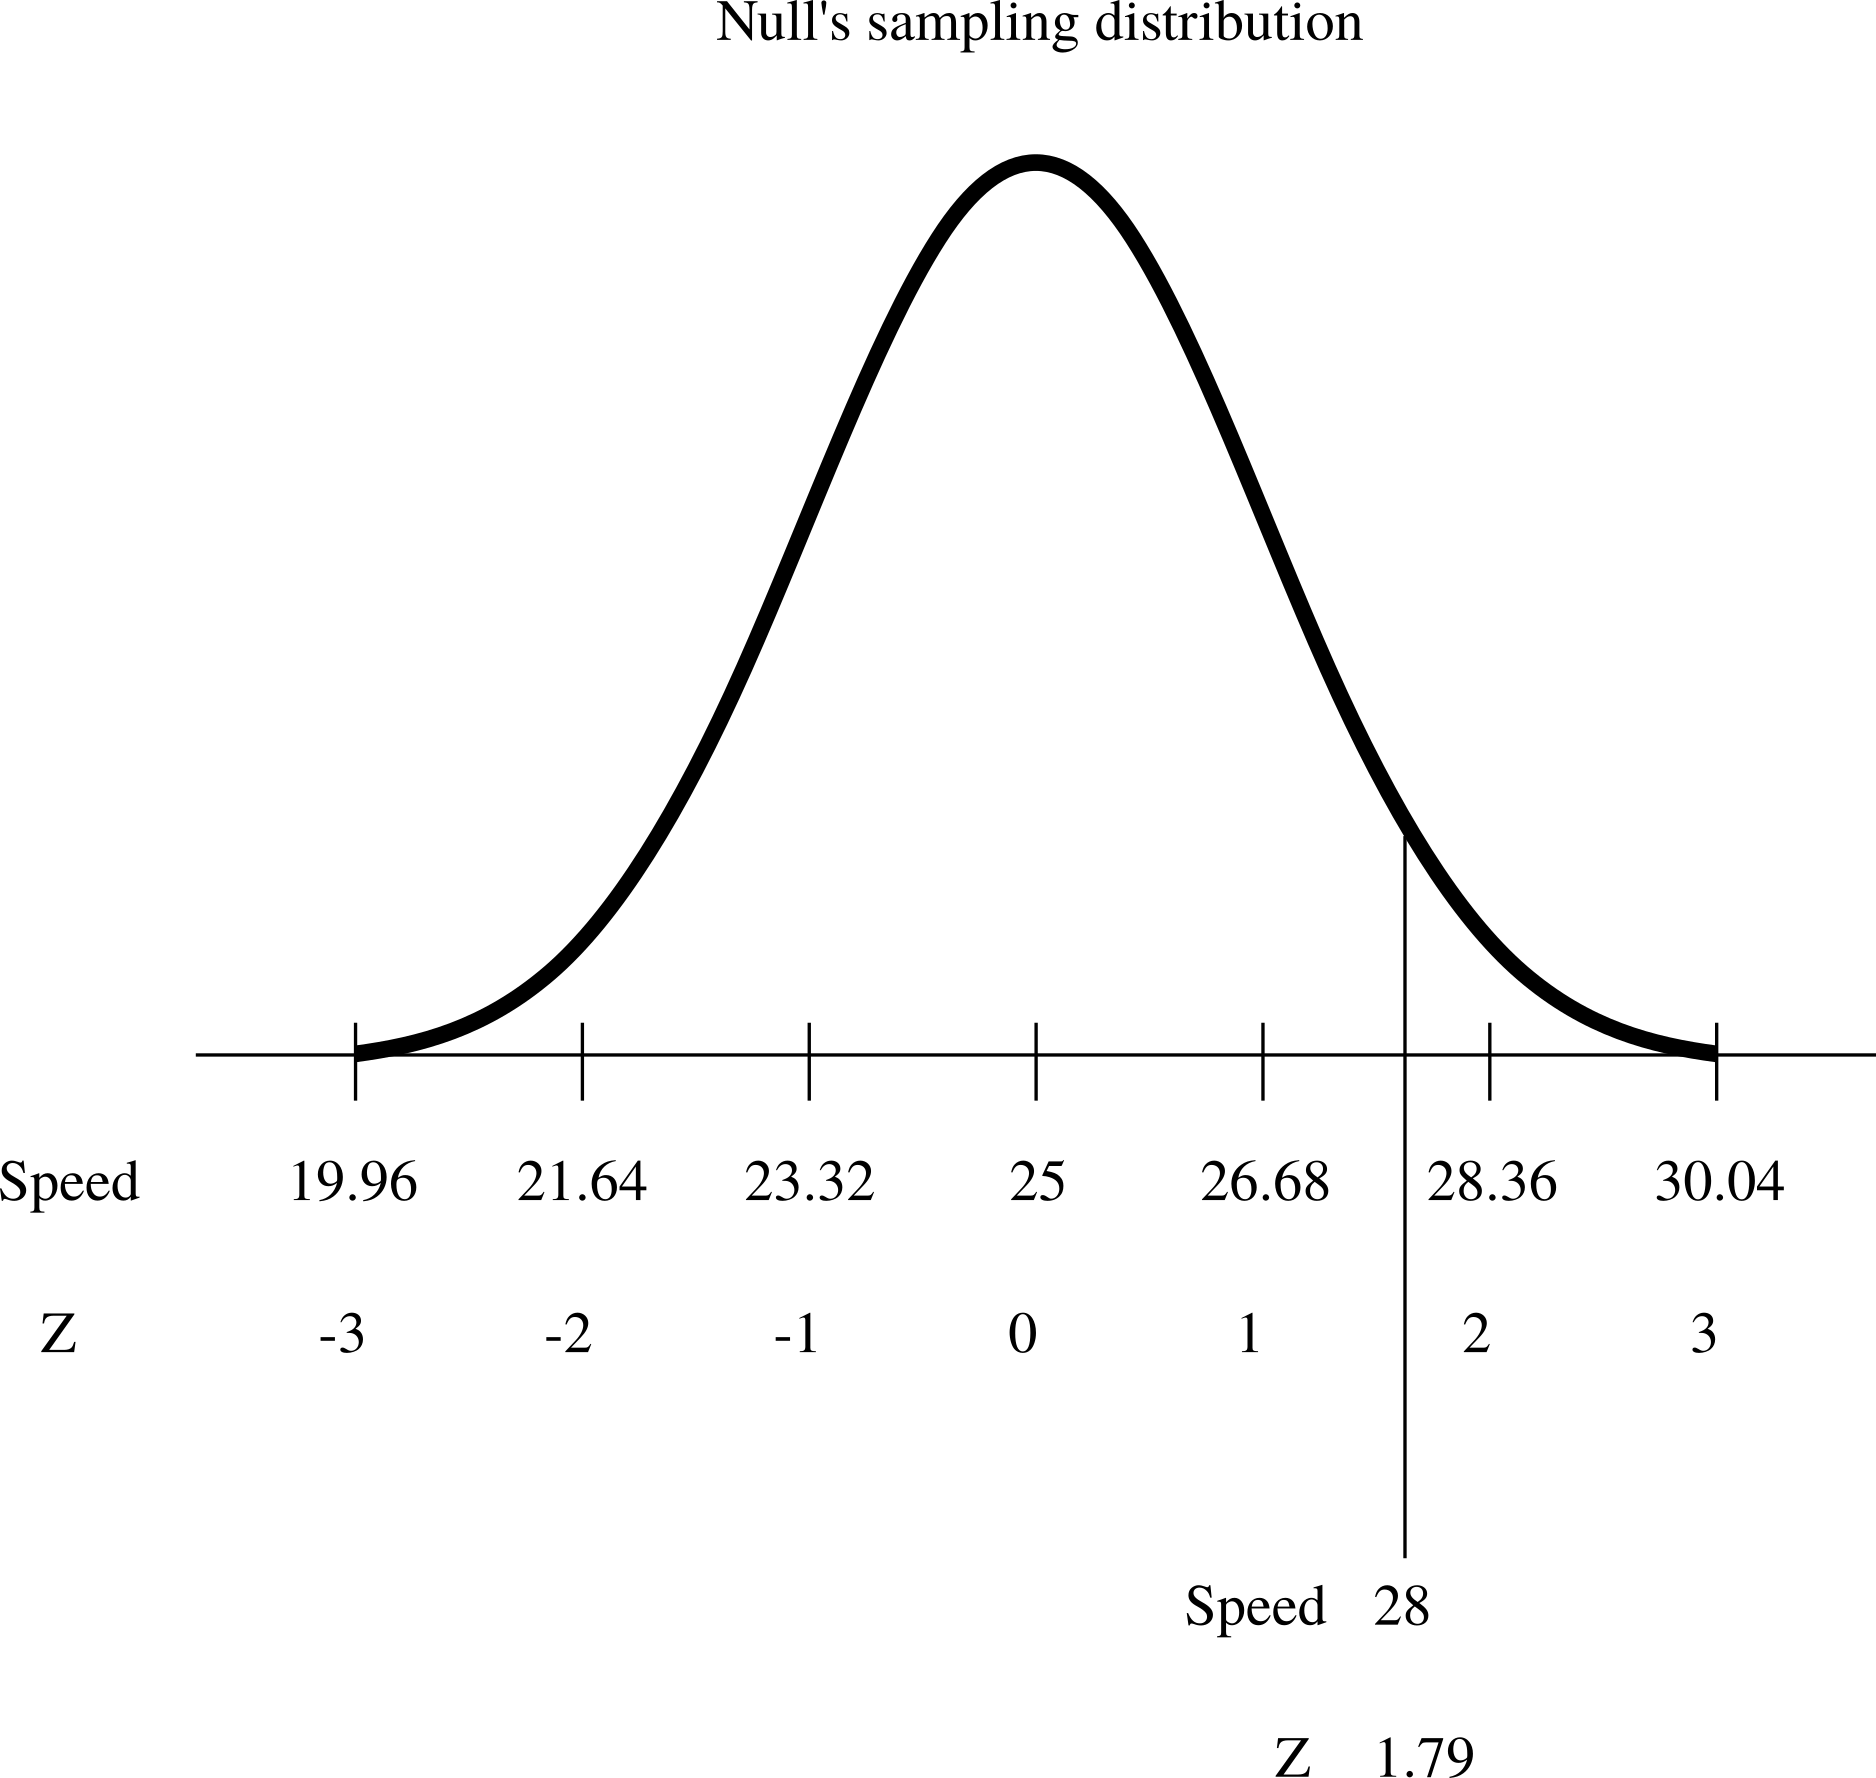
\includegraphics[width=0.9\textwidth]{4-3_hyp_test/figures/null.png}
\end{center} \pause
}
{
   In this case, the test statistic is $z = \frac{28-25}{1.68} = 1.79$. \pause
   \vspace{10pt}
      
   We quantify how unusual this is with a $p$-value.
}

\end{frame}

%%%%%%%%%%%%%%%%%%%%%%%%%%%%%%%%%%%

\begin{frame}
\frametitle{p-values}

\begin{itemize}

\item We then use this test statistic to calculate the \hl{p-value}, the probability of observing data at least as favorable to the alternative hypothesis as our current data set, if the null hypothesis were true.

\pause

\item If the p-value is \hl{low} (lower than the significance level, $\alpha$, which is usually 5\%) we say that it would be very unlikely to observe the data if the null hypothesis were true, and hence \hl{reject $H_0$}.

\pause

\item If the p-value is \hl{high} (higher than $\alpha$) we say that it is likely to observe the data even if the null hypothesis were true, and hence \hl{do not reject $H_0$}.

\end{itemize}

\end{frame}

%%%%%%%%%%%%%%%%%%%%%%%%%%%%%%%%%%%%

\begin{frame}
\frametitle{Speeding example}
$p$-value: The probability of observing data at least as favorable to $H_A$ as our current data set (a sample mean greater than 28) if in fact $H_0$ were true (the population mean was 25).
\begin{center}
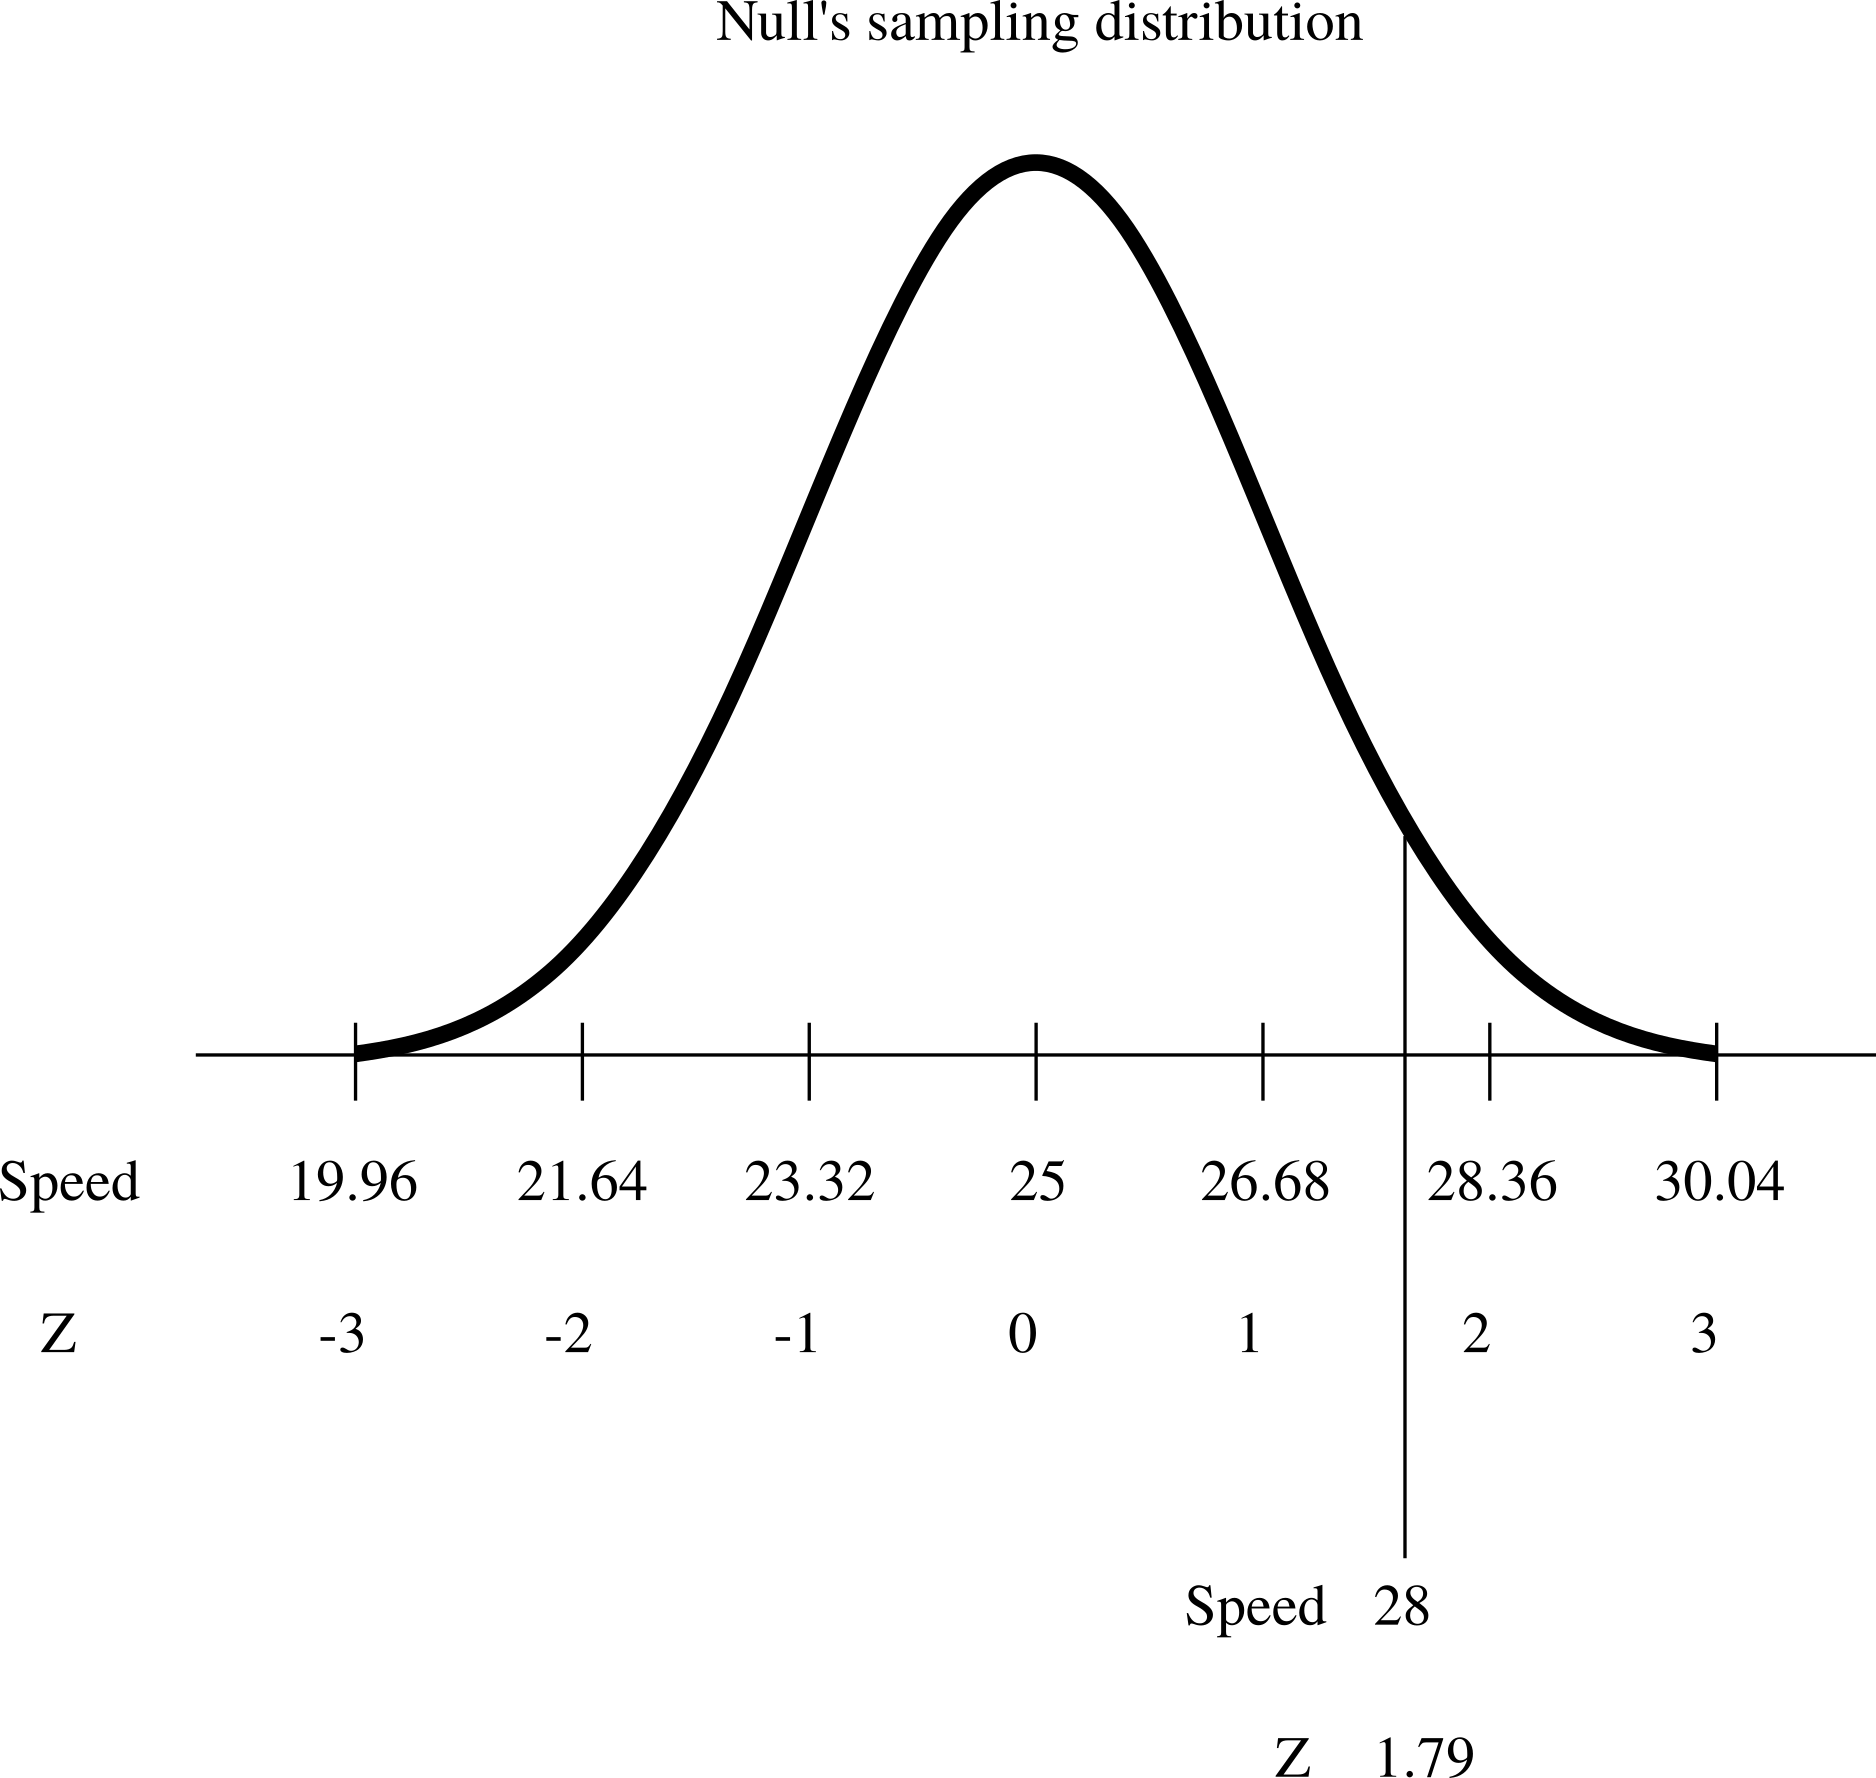
\includegraphics[width=0.4\textwidth]{4-3_hyp_test/figures/null.png}
\end{center} 
\pause

$$P(\bar{x} > 28 | \mu = 25) = P(Z > 1.79) = 0.0367 $$

\end{frame}

%%%%%%%%%%%%%%%%%%%%%%%%%%%%%%%%%%

\begin{frame}
\frametitle{Making a decision}

\begin{itemize}

\item p-value = 0.0367

\pause

\begin{itemize}
\item If the true average speed 25, there is only 3.67\% chance of observing a random sample of 80 drivers who on average drive 28 mph or more.
\pause
\item This is a pretty low probability for us to think that a sample mean of 28 mph is likely to happen simply by chance.
\end{itemize}

\pause
\item Since p-value is \orange{low} (lower than 5\%) we \orange{reject $H_0$}.

\pause
\item The data provide convincing evidence that cars speed.

\pause
\item The difference between the null value of 25 mph and observed sample mean of 28 mph is \orange{not due to chance} or sampling variability.

\end{itemize}

\end{frame}

%%%%%%%%%%%%%%%%%%%%%%%%%%%%%%%%%%%%

\begin{frame}
\frametitle{}

\pq{{\footnotesize A poll by the National Sleep Foundation found that college students average about 7 hours of sleep per night. A sample of 169 college students taking an introductory statistics class yielded an average of 6.88 hours, with a standard deviation of  0.94 hours. Assuming that this is a random sample representative of all college students {\scriptsize \textit{(bit of a leap of faith?)}}, a hypothesis test was conducted to evaluate if college students on average sleep \emph{less than} 7 hours per night. The p-value for this hypothesis test is 0.0485. Which of the following is correct?}}

\begin{enumerate}[(a)] \small
\item Fail to reject $H_0$, the data provide convincing evidence that college students sleep less than 7 hours on average.
\solnMult{ Reject $H_0$, the data provide convincing evidence that college students sleep less than 7 hours on average. }
\item Reject $H_0$, the data prove that college students sleep more than 7 hours on average.
\item Fail to reject $H_0$, the data do not provide convincing evidence that college students sleep less than 7 hours on average.
\item Reject $H_0$, the data provide convincing evidence that college students in this sample sleep less than 7 hours on average.
\end{enumerate}

\end{frame}

%%%%%%%%%%%%%%%%%%%%%%%%%%%%%%%%%

\subsection{Two-sided hypothesis testing with p-values}

%%%%%%%%%%%%%%%%%%%%%%%%%%%%%%%%%

\begin{frame}
\frametitle{Two-sided hypothesis testing with p-values}

\begin{itemize}

\item If the research question was ``Do the data provide convincing evidence that the average amount of sleep college students get per night is \orange{different} than the national average?", the alternative hypothesis would be different.
\begin{align*}
H_0&: \mu = 7 \\
H_A&: \mu \orange{~$\ne$~} 7
\end{align*}

\pause

\item Hence the p-value would change as well:
\twocol{0.55}{0.45}
{
\begin{center}
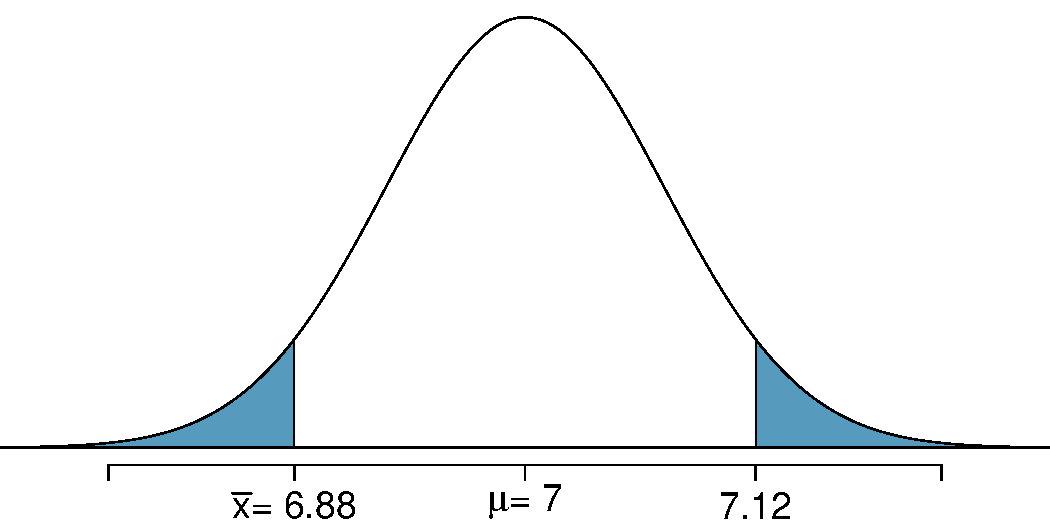
\includegraphics[width=\textwidth]{4-3_hyp_test/figures/sleep/sleep_pval_ts}
\end{center}
}
{
p-value \\
$= 0.0485 \times 2$ \\
$= 0.097$
}

\end{itemize}

\end{frame}

%%%%%%%%%%%%%%%%%%%%%%%%%%%%%%%%%%%%

\subsection{Decision errors}

%%%%%%%%%%%%%%%%%%%%%%%%%%%%%%%%%%%%

\begin{frame}
\frametitle{Decision errors}

\begin{itemize}

\item Hypothesis tests are not flawless.

\item In the court system innocent people are sometimes wrongly convicted and the guilty sometimes walk free.

\item Similarly, we can make a wrong decision in statistical hypothesis tests as well. 

\item The difference is that we have the tools necessary to quantify how often we make errors in statistics.

\end{itemize}

\end{frame}

%%%%%%%%%%%%%%%%%%%%%%%%%%%%%%%%%%%%

\begin{frame}
\frametitle{Decision errors (cont.)}

There are two competing hypotheses: the null and the alternative. In a hypothesis test, we make a decision about which might be true, but our choice might be incorrect. \\

\pause

\begin{center}
\begin{tabular}{l l | c c}
\multicolumn{2}{c}{} & \multicolumn{2}{c}{\textbf{Decision}} \\
& & fail to reject $H_0$ &  reject $H_0$ \\
  \cline{2-4}
& $H_0$ true & \onslide<3->{\green{$\checkmark$}} &  \onslide<5->{\orange{Type 1 Error}} \\
\raisebox{1.5ex}{\textbf{Truth}} & $H_A$ true & \onslide<6->{\orange{Type 2 Error}} & \onslide<4->{\green{$\checkmark$}} \\
  \cline{2-4}
\end{tabular}
\end{center}

\begin{itemize}
\item \onslide<5->{A \hl{Type 1 Error} is rejecting the null hypothesis when $H_0$ is true.}

\item \onslide<6->{A \hl{Type 2 Error} is failing to reject the null hypothesis when $H_A$ is true.}

\item \onslide<7->{We (almost) never know if $H_0$ or $H_A$ is true, but we need to consider all possibilities.}

\end{itemize}

\end{frame}

%%%%%%%%%%%%%%%%%%%%%%%%%%%%%%%%%%%%

\begin{frame}
\frametitle{Hypothesis Test as a trial}

If we again think of a hypothesis test as a criminal trial then it makes sense to frame the verdict in terms of the null and alternative hypotheses:
\begin{align*}
H_0&:\text{ Defendant is innocent} \\
H_A&:\text{ Defendant is guilty}
\end{align*}

Which type of error is being committed in the following circumstances?

\begin{itemize}
\item Declaring the defendant innocent when they are actually guilty
\soln{\only<2->{\begin{center}\hl{Type 2 error}\end{center}}}
\item Declaring the defendant guilty when they are actually innocent
\soln{\only<3->{\begin{center}\hl{Type 1 error}\end{center}}}
\end{itemize}

\only<4->{Which error do you think is the worse error to make?}
\only<5>{\begin{center}{\footnotesize ``better that ten guilty persons escape than that one innocent suffer''\\ -- William Blackstone}\end{center}}
\end{frame}

%%%%%%%%%%%%%%%%%%%%%%%%%%%%%%%%%%%%

\begin{frame}
\frametitle{Type 1 error rate}

\begin{itemize}

\item As a general rule we reject $H_0$ when the p-value is less than 0.05, i.e. we use a \hl{significance level} of 0.05, \mathhl{\alpha = 0.05}.

\pause

\item This means that, for those cases where $H_0$ is actually true, we do not want to incorrectly reject it more than 5\% of those times. 

\pause

\item In other words, when using a 5\% significance level there is about 5\% chance of making a Type 1 error if the null hypothesis is true.
\[ \mathhl{ P(\text{Type 1 error} | \text{$H_0$ true}) = \alpha } \]

\pause

\item This is why we prefer small values of $\alpha$ -- increasing $\alpha$ increases the Type 1 error rate.

\end{itemize}

\end{frame}

%%%%%%%%%%%%%%%%%%%%%%%%%%%%%%%%%%%%

\subsection{Choosing a significance level}

%%%%%%%%%%%%%%%%%%%%%%%%%%%%%%%%%%%%

\begin{frame}
\frametitle{Choosing a significance level}

\begin{itemize}

\item Choosing a significance level for a test is important in many contexts, and the traditional level is 0.05. However, it is often helpful to adjust the significance level based on the application. 

\item We may select a level that is smaller or larger than 0.05 depending on the consequences of any conclusions reached from the test.

\item If making a Type 1 Error is dangerous or especially costly, we should choose a small significance level (e.g. 0.01). Under this scenario we want to be very cautious about rejecting the null hypothesis, so we demand very strong evidence favoring $H_A$ before we would reject $H_0$.

\item If a Type 2 Error is relatively more dangerous or much more costly than a Type 1 Error, then we should choose a higher significance level (e.g. 0.10). Here we want to be cautious about failing to reject $H_0$ when the null is actually false.

\end{itemize}

\end{frame}

%%%%%%%%%%%%%%%%%%%%%%%%%%%%%%%%%%%%

\subsection{Recap}

%%%%%%%%%%%%%%%%%%%%%%%%%%%%%%%%%%%%

\begin{frame}

\vfill

\textit{the next two slides are provided as a brief summary of hypothesis testing...}

\vfill

\end{frame}

%%%%%%%%%%%%%%%%%%%%%%%%%%%%%%%%%%%%

\begin{frame}
\frametitle{Recap: Hypothesis testing framework}

\begin{enumerate}

\item Set the hypotheses.

\item Check assumptions and conditions.

\item Calculate a \hl{test statistic} and a p-value.

\item Make a decision, and interpret it in context of the research question.

\end{enumerate}

\end{frame}

%%%%%%%%%%%%%%%%%%%%%%%%%%%%%%%%%%%

\begin{frame}
\frametitle{Recap: Hypothesis testing for a population mean}

\begin{enumerate}

\item Set the hypotheses
\begin{itemize}
\item $H_0: \mu = null~value$
\item $H_A: \mu <$ or $>$ or $\ne null~value$
\end{itemize}

\item Calculate the point estimate

\item Check assumptions and conditions
\begin{itemize}
\item Independence: random sample/assignment, 10\% condition when sampling without replacement
\item Normality: nearly normal population or $n \ge 30$, no extreme skew -- or use the t distribution
\end{itemize}

\item Calculate a \hl{test statistic} and a p-value (draw a picture!)
\[ Z = \frac{\bar{x} - \mu}{SE},~where~SE = \frac{s}{\sqrt{n}} \]

\item Make a decision, and interpret it in context
\begin{itemize}
\item If p-value $< \alpha$, reject $H_0$, data provide evidence for $H_A$
\item If p-value $> \alpha$, do not reject $H_0$, data do not provide evidence for $H_A$
\end{itemize}

\end{enumerate}

\end{frame}

%%%%%%%%%%%%%%%%%%%%%%%%%%%%%%%%%%%%
